\part*{Annexes}
\addcontentsline{toc}{chapter}{Annexes} % Ajout dans la table des matieres




\subsection* {Tableau comparatif des différents casques EEG proposés sur le marché}

\begin{figure}[h]
	\centering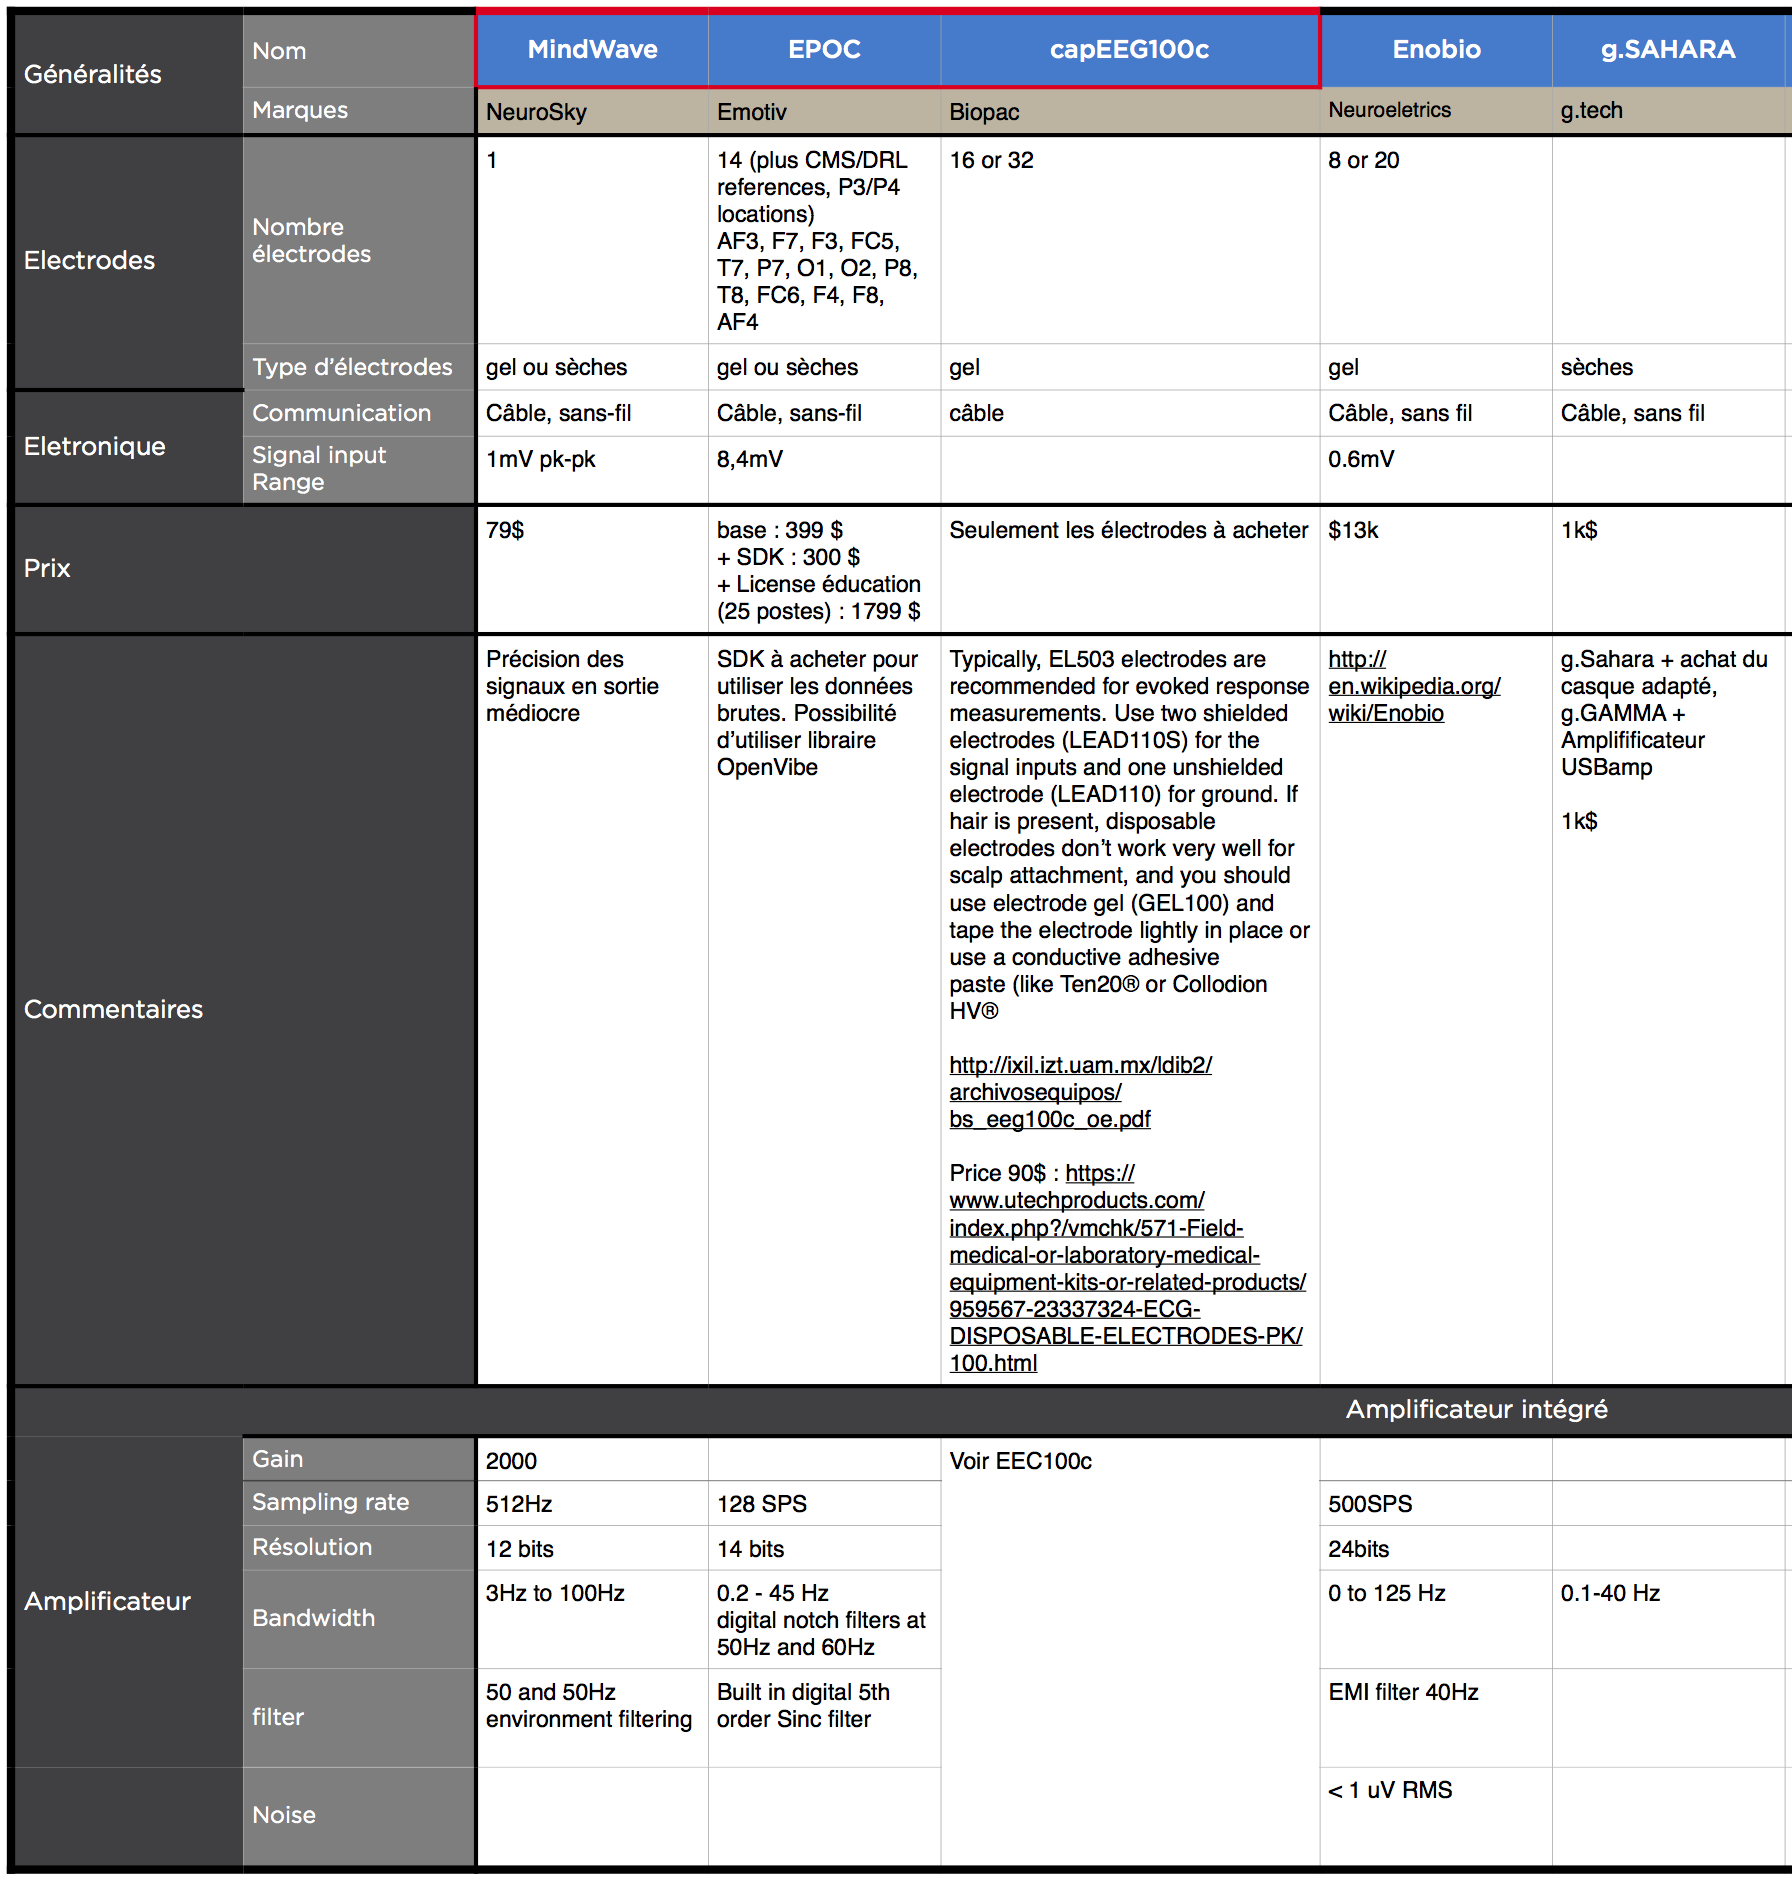
\includegraphics[width=17cm, angle=0]{images/ComparaisonCasques.jpg}
\end{figure}




\newpage
\subsection* {Tableau comparatif des différents amplificateurs proposés sur le marché}

\begin{figure}[h]
	\centering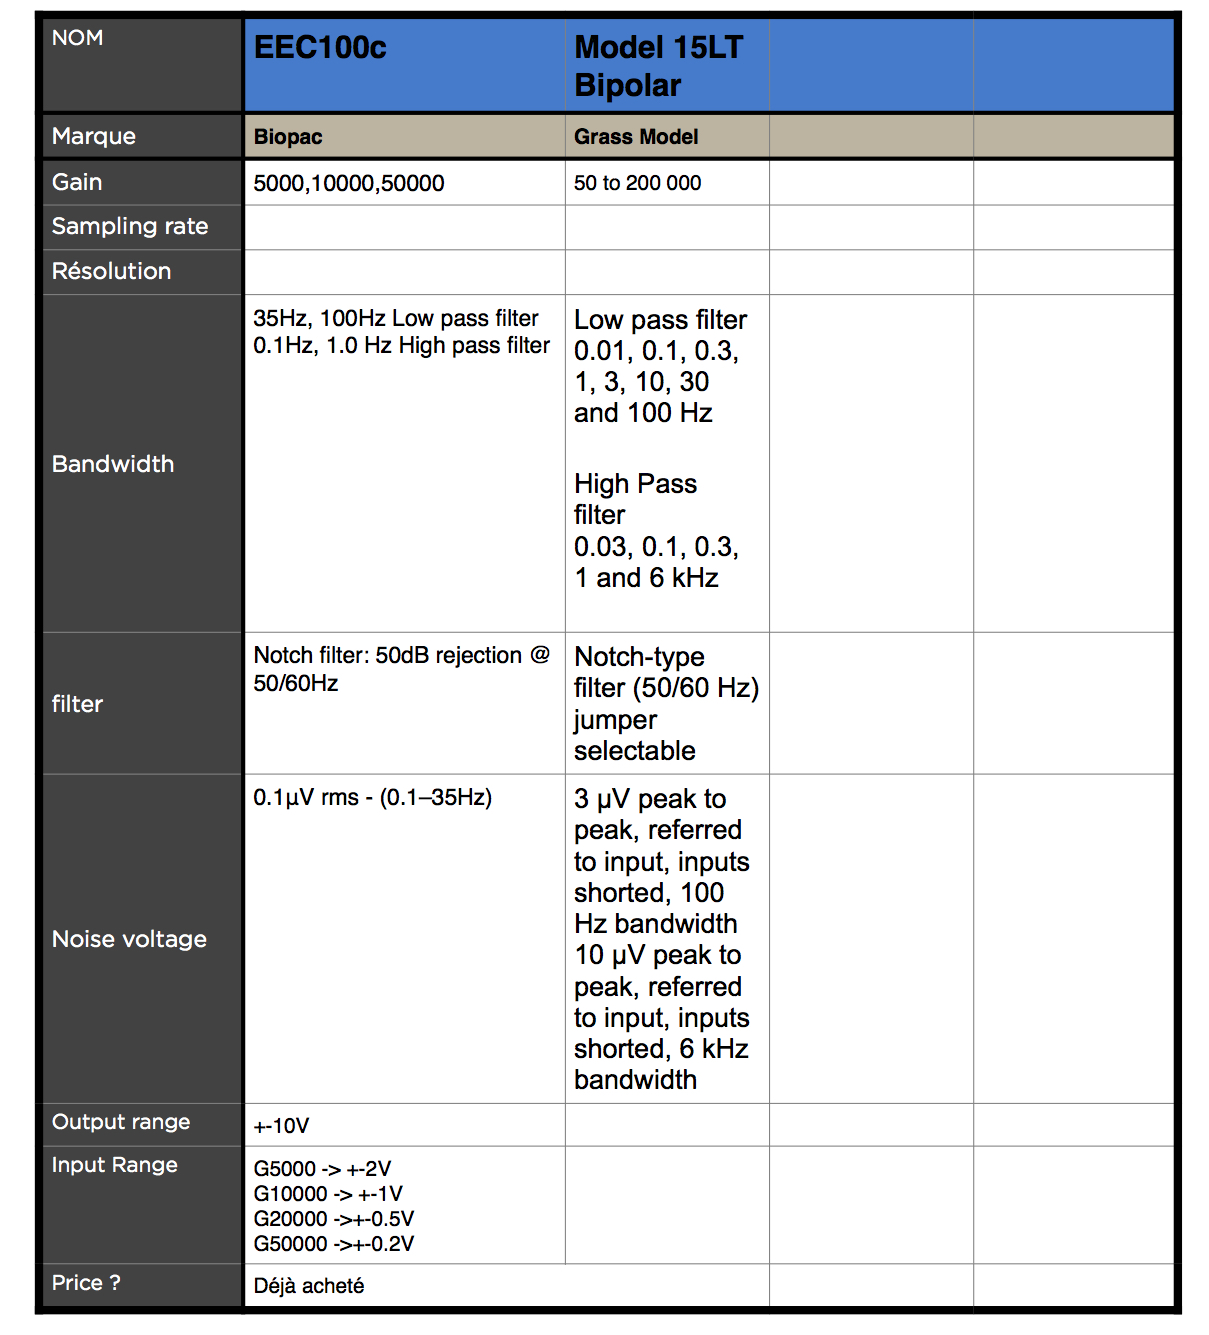
\includegraphics[width=17cm, angle=0]{images/ComparaisonAmpli.jpg}
\end{figure}



\newpage
\subsection* {Carte heuristique}

\begin{figure}[h]
	\centering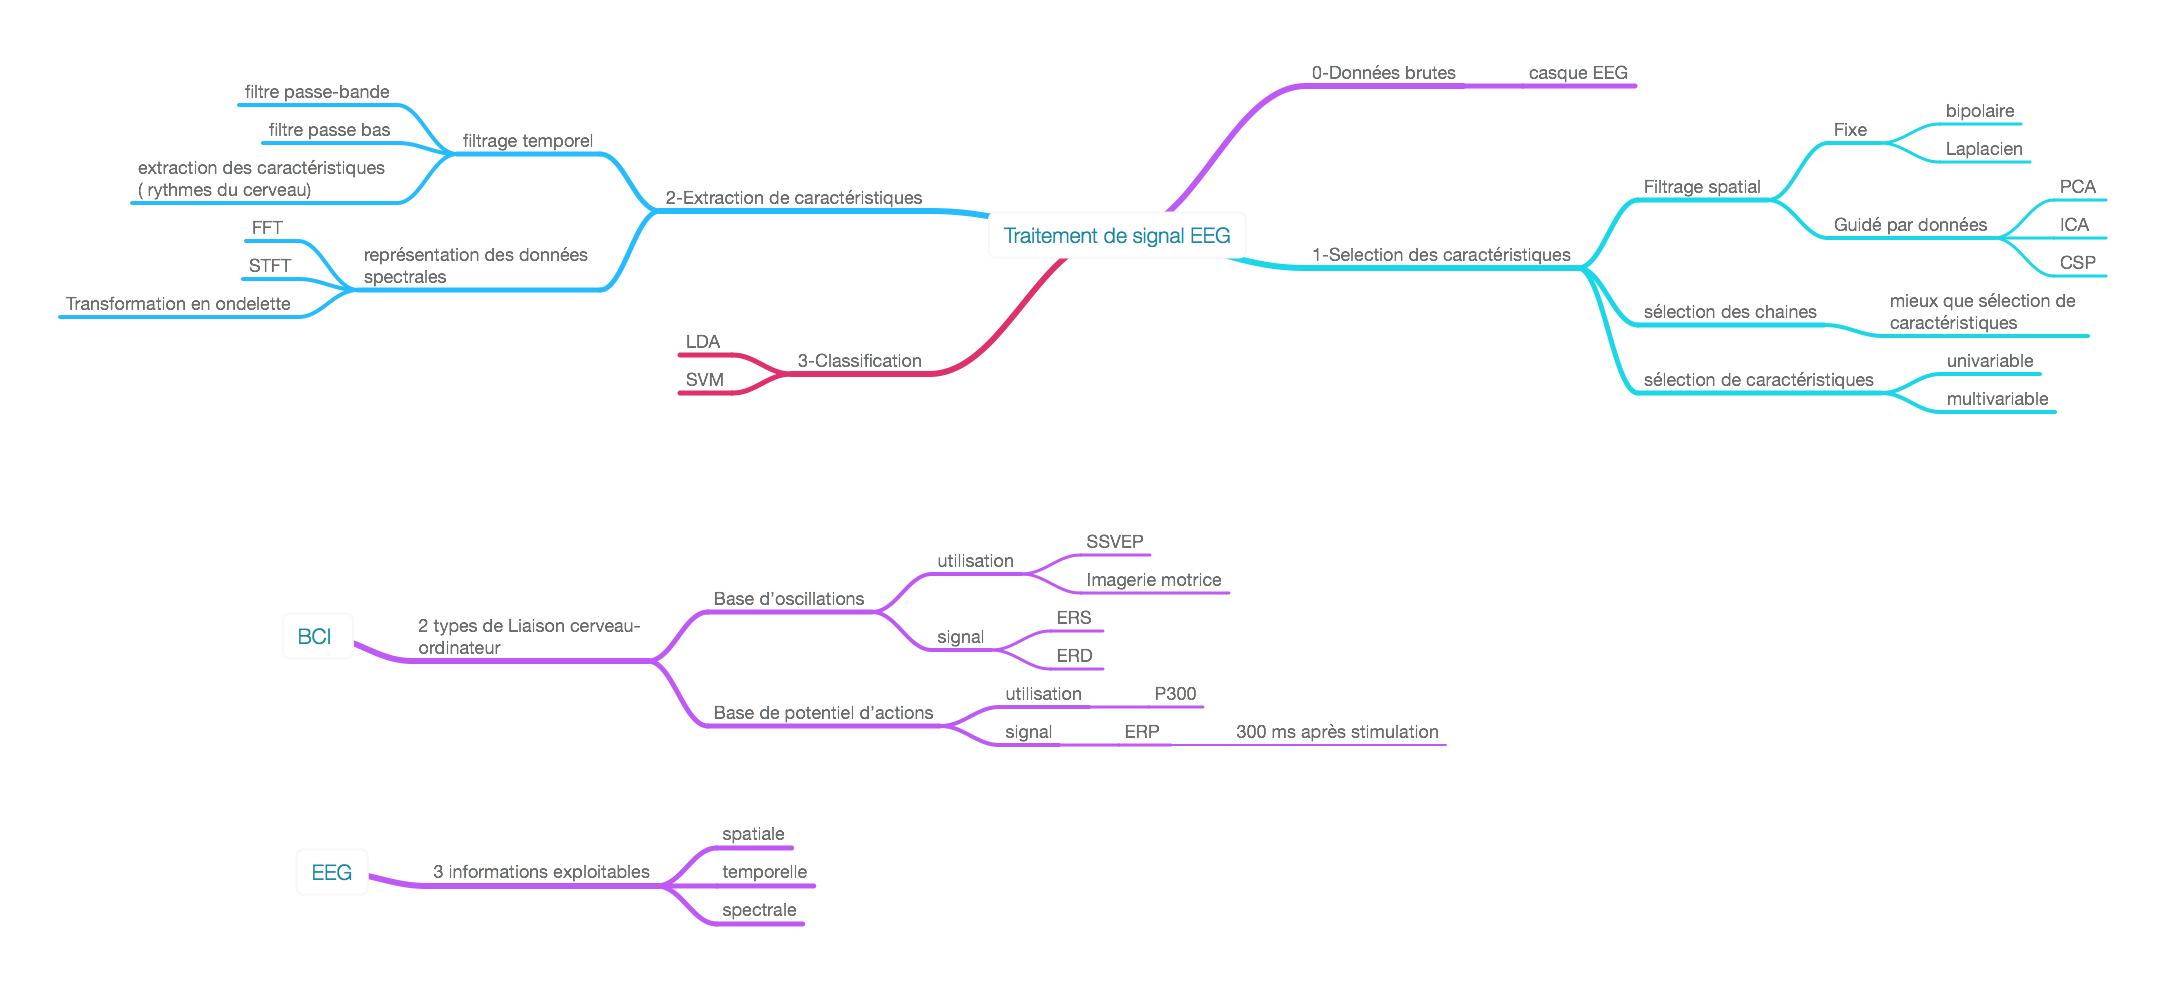
\includegraphics[width=19cm,angle=90,]{images/CarteHeuristiqueSignalProcessing.png}
\end{figure}
\newpage
\subsubsection{Sujet filtrage ICA}

\begin{verbatim}
%##########################################################################
%#####     SUJET DE TP DE COURS DE TRAITEMENT DE SIGNAL AVANCE    #########
%#######################   ICA     ########################################
%### Florian Lepont, Romain Richard######### Avril 2015####################

close all
clear all

% LECTURE DES DONNEES A PARTIR DU FICHIER CSV
donnees_eeg = lecture_csv('données_entrée.csv')

% ANALYSE EN COMPOSANTES INDEPENDANTES
sources = ica(donnees_eeg) % on récupère les données du fichier

% AFFICHAGE DES DONNNEES
subplot(2,2,1) 
plot(donnees_eeg')
xlabel('temps (s)')
ylabel('amplitude (mV)')

subplot(2,2,2)
plot(sources')
xlabel('temps (s)')
ylabel('amplitude (mV)')

subplot(2,2,3)
hist(donnees_eeg')
xlabel('amplitude (mV)')
ylabel('nombres de données')

subplot(2,2,4)
xlabel('temps (s)')
ylabel('amplitude du signal (mV)')

hist(sources')
xlabel('amplitude (mV)')
ylabel('nombres de données')

% CREATION DU FICHIER DE SORTIE
ecriture_csv( 'données_entrée.csv', 'données_EEG_sortie.csv', sources)
\end{verbatim}



\newpage
\subsubsection{Correction filtrage ICA}

\begin{verbatim}
%##########################################################################
%#####     CORRECTION FONCTION COURS TRAITEMENT SIGNAL AVANCE #############
%#######################   ICA     ########################################
%### Florian Lepont, Romain Richard######### Avril 2015####################

% Bibliographie : "A Tutorial on Independant Component Analysis" de Jonathon Shlens

function sources = ica(donnees)
% Analyse en composantes indépendantes.
% ENTREE : données à traiter
% SORTIE : Matrice de transformation linéaire, signaux sources calculés

[M,N] = size(donnees);

%  Translation de la moyenne des données vers 0.
mn = mean(donnees,2);
donnees = donnees - repmat(mn,1,N);

% Calcul de la matrice de covariance
covariance = 1 / (N-1) * (donnees * donnees');

% Calcul des valeurs propres et des vecteurs propres de la matrice de
% covariance.
[E,D] = eig(covariance);

%Calcul des données décoréllées et normalisation.
X = sqrtm(pinv(D))*E'*donnees;

%Calcul de la décomposition en valeurs singulières. (calcul de la
%transformation linéraire - rotation - V).
[V,s,u] = svd((repmat(sum(X.*X,1),M,1).*X)*X');

%Calcul de la transformation linéaire W
W = V * sqrtm(pinv(D)) * E';

%Calcul des signaux sources
sources = W * donnees;
\end{verbatim}


\newpage
\subsubsection{Sujet filtrage PCA}

\begin{verbatim}
%##########################################################################
%#######   SUJET DE TP DE COURS DE TRAITEMENT DE SIGNAL AVANCE    #########
%#########################   PCA  #########################################
%### Florian Lepont, Romain Richard######### Avril 2015####################

close all
clear all

% LECTURE DES DONNEES A PARTIR DU FICHIER CSV
donnees_eeg = lecture_csv('données_entrée.csv')

% ANALYSE EN COMPOSANTES PRINCIPALES
% On récupère les données du fichier
[signaux_pca,composantes_principales,valeurs_propres] = pca(donnees_eeg) 

% AFFICHAGE DES DONNNEES
subplot(2,2,1) 
plot(donnees_eeg')
xlabel('temps (s)')
ylabel('amplitude (mV)')

subplot(2,2,2)
plot(signaux_pca')
xlabel('temps (s)')
ylabel('amplitude (mV)')

subplot(2,2,3)
hist(donnees_eeg')
xlabel('amplitude (mV)')
ylabel('nombres de données')

subplot(2,2,4)
xlabel('temps (s)')
ylabel('amplitude du signal (mV)')

hist(signaux_pca')
xlabel('amplitude (mV)')
ylabel('nombres de données')

% CREATION DU FICHIER DE SORTIE
ecriture_csv( 'données_entrée.csv', 'données_EEG_sortie.csv', signaux_pca)
\end{verbatim}


\newpage
\subsubsection{Correction filtrage PCA}

\begin{verbatim}
%##########################################################################
%#####     CORRECTION FONCTION COURS TRAITEMENT SIGNAL AVANCE #############
%#######################   PCA     ########################################
%### Florian Lepont, Romain Richard######### Avril 2015####################

% Bibliographie : "A Tutorial on Principal Component Analysis" de Jonathon Shlens

function [signaux,composantes_principales,valeurs_propres] = pca(donnees)
% Analyse en composantes principales.
% ENTREE : données à traiter
% SORTIE : Signaux décorrélés, vecteur des composantes principales,
% vecteurs_propres

[M,N] = size(donnees);

%  Translation de la moyenne des données vers 0.
mn = mean(donnees,2);
donnees = donnees - repmat(mn,1,N);

% Calcul de la matrice de covariance
covariance = 1 / (N-1) * (donnees * donnees');

% Calcul des valeurs propres et des vecteurs propres de la matrice de
% covariance. Les vecteurs propres en sortie correspondent aux
% composantes principales.
[composantes_principales,valeurs_propres] = eig(covariance);

% Extraction des valeurs propres de la matrice vers un vecteur
valeurs_propres = diag(valeurs_propres);

% Trie des valeurs propres par ordre décroissant
[junk, indices] = sort(-1*valeurs_propres);
valeurs_propres = valeurs_propres(indices);
composantes_principales = composantes_principales(:,indices);

% On réalise la transformation linéaire des données d'entrée
signaux = composantes_principales'* donnees;
\end{verbatim}




\newpage
\subsection*{Lecture CSV}

\begin{verbatim}
%##########################################################################
%#####     FONCTION LECTURE D UNE FICHIER CSV    ##########################
%#######################   CSV     ########################################
%### Florian Lepont, Romain Richard######### Avril 2015####################

function [donnees_eeg] = lecture_csv( fichier_entree )
% Fonction lecture vers un fichier csv. La fonction permet de lire
% les données EEG contenues dans le ficher csv 'fichier_entree'. 

% EXTRACTION DES DONNEES EEG 
% Extraction des données EEG à partir du fichier CSV
% Suppression des infos temps et frequence d'échantillonnage afin de ne conserver 
% que les données des signaux
donnees_eeg(:,1) = [] 			
donnees_eeg(:,end) = []     
% Calcul de la transposée                                                
donnees_eeg = donnees_eeg'			

end
\end{verbatim}




\newpage
\subsection*{Écriture CSV}

\begin{verbatim}
%##########################################################################
%#####     FONCTION ECRITURE D UNE FICHIER CSV   ##########################
%#######################   CSV     ########################################
%### Florian Lepont, Romain Richard######### Avril 2015####################

function [] = ecriture_csv( fichier_entree, fichier_sortie, donnees)
% Fonction ecriture vers un fichier csv. La fonction permet d'ecrire
% vers le ficher csv 'fichier_sortie'. Pour cela, il récupère les 
% informations temps, fréq_echantill, colonnes et lignes à partir du
% fichier csv 'fichier_entree', généré par OpenViBE. 

% EXTRACTION DES DONNEES EEG ET CARACTERISTIQUES ACQUISITION
% Extraction des données EEG
donnees_eeg = csvread(fichier_entree,1,0);        
% Extraction de la taille du tableau de données                          
[lignes,colonnes] = size(donnees_eeg)        
% La première colonne du fichier csv correspond aux échantillons temporels                               
temps = donnees_eeg(:,1)           
% La valeurs de la dernière colonne du fichier csv correpond à la fréquence
% d'échantillonnage                                          
freq_echant = donnees_eeg(1,end)                                           

% EXTRACTION DU NOM DES VALEURS A PARTIR DU FICHIER D'ENTREE
% Ouverture du fichier csv 
fid = fopen(fichier_entree,'r');      
% On récupère les données du fichier                                      
C = textscan(fid, repmat('%s',1,colonnes), 'delimiter',',', 'CollectOutput',true); 
C = C{1};
% extraction de la première ligne du fichier, comprenant le nom des variables
nom_valeurs = C(1,:);                                                       
fclose(fid);

% CREATION DU FICHIER DE SORTIE
% Ouverture du nouveau fichier
fid1 = fopen(fichier_sortie,'w');                                           

% Concaténations des données temps et fréquence d'échantillonnage avec 
% les nouvelles valeurs décoréllées
donnees_csv = horzcat(temps, donnees')                                      
donnees_csv(:,end+1) = zeros;
donnees_csv(1,end) = freq_echant

headerFmt = repmat('%s,',1,colonnes-1); 
numFmt = repmat('%f,',1,colonnes-1);
% Écriture de l'en-tête du csv (nom des variables)
fprintf(fid1,[headerFmt,'%s\n'],nom_valeurs{1,:});    
% Écriture des données                      
fprintf(fid1,[numFmt,'%f\n'],donnees_csv');                                 

fclose(fid1)
end
\end{verbatim}


\newpage
\thispagestyle{fancy}

\begin{center}
\huge\textbf{GEI 723 : Travail pratique}
\bigbreak
\LARGE\textbf{Visualisation de signaux EEG et de l'activité cérébrale}
\bigbreak
\end{center}

\normalsize

On vous propose à travers ce travail pratique de vous familiariser avec les aspects théoriques et techniques d'une interface cerveau-ordinateur (BCI). Celle que nous vous demandons d'étudier a été mise au point sous le logiciel libre de droit OpenViBE.

\newpage
\section*{Interface cerveau-ordinateur}

L'expérience que l'on vous propose d'étudier s'appuie sur la méthode d'imagerie motrice, qui consiste à imaginer le mouvement de différentes parties du corps. Cela résulte en l'activation du cortex sensorimoteur qui module certains rythmes du cerveau. Ces variations peuvent être détectées par des électrodes EEG. L'interface cerveau-ordinateur en déduit les intentions de l'utilisateur à partir de ces signaux. Dans notre cas, celle-ci doit être capable de déterminer si l'utilisateur pense à un mouvement de sa main droite ou de sa main gauche.

La chaîne de traitement des signaux EEG de l'interface cerveau-ordintaeur se compose en 5 étapes (Figure	\ref{fig:interface_travail_ov_2}) : 

\begin{enumerate}
	\item \textbf{L'acquisition des données.} En temps normal, on récupère en temps réel les données directement issues d'un casque EEG (par exemple le casque EPOC). Comme vous ne possédez pas ce genre de casque, on vous fournit un fichier .ov contenant des signaux EEG pré-enregistrés d'une personne pensant aléatoirement à sa main gauche ou droite.
	\smallbreak
	\item \textbf{Filtrage temporel.} Ce filtrage permet d'extraire les rythmes du cerveau qui nous intéressent.
	\smallbreak
	\item \textbf{Filtrage spatial CSP.} Permet de réduire la quantité d'informations à traiter en réalisant une décorrélation et en pondérant certaines des sorties du casque. 
	\smallbreak
	\item \textbf{Analyse spectrale.} Réalise une analyse spectrale via une transformée de Fourier.
	\smallbreak
	\item \textbf{Classification.} Effectue une classification des caractéristiques à son entrée afin de déterminer à quelle main pensait l'utilisateur à un instant donné. 
\end{enumerate}

Le filtre spatial et le classificateur nécessitent d'être préalablement entrainés grâce à d'autres scénarios, générant alors un fichier de configuration pour ces deux blocs ("Classifier.cfg" et "csp-spatial-filter.cfg" ). On vous fournit ici directement ces fichiers de configuration.

\begin{figure}[h]
	\centering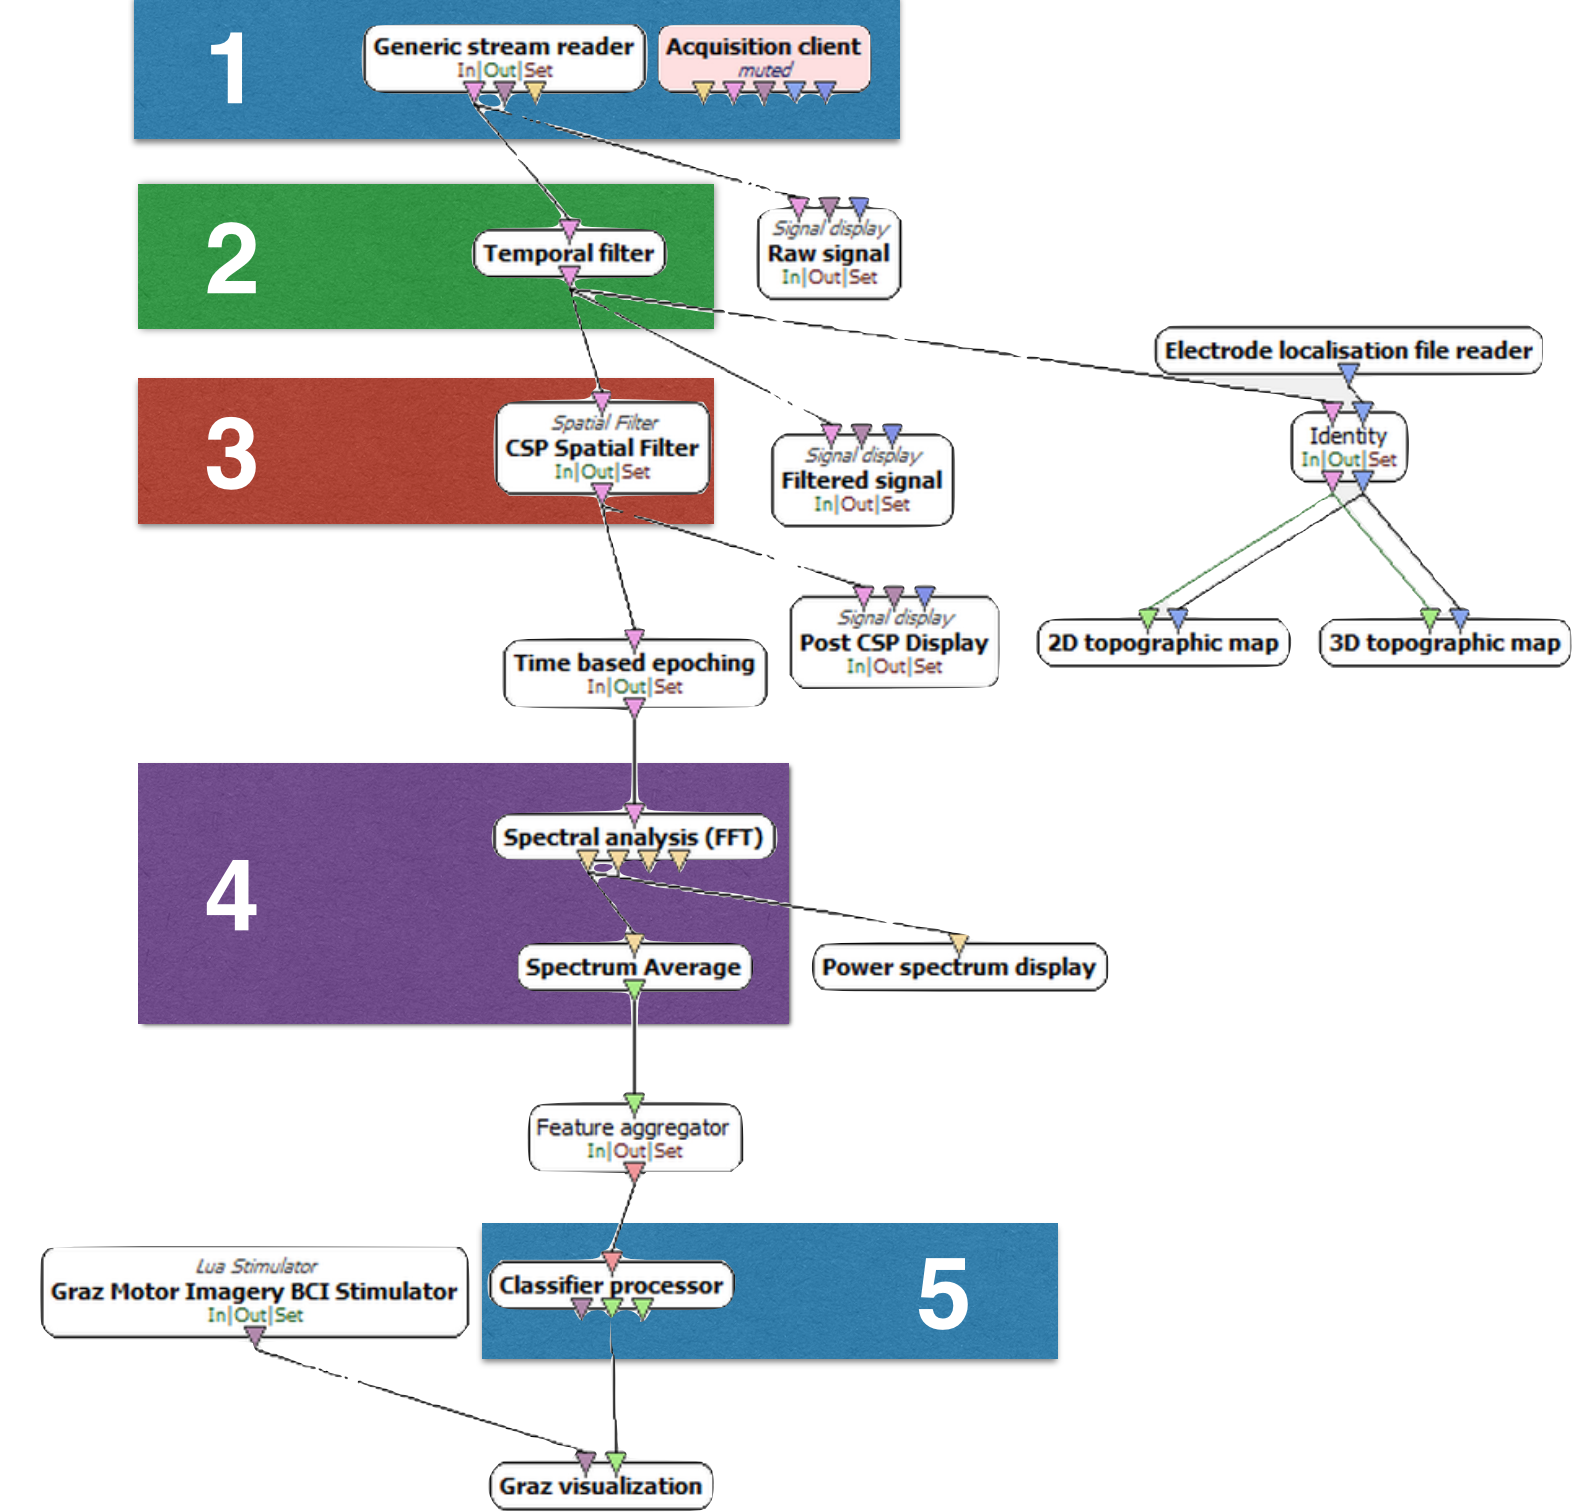
\includegraphics[height=12cm]{images/scenario_neuro_color.png}
	\caption{Traitement des signaux EEG sous OpenViBE.}
	\label{fig:interface_travail_ov_2}
\end{figure}


Voici la description des différents blocs utilisés dans ce scénario :

\subsubsection*{Traitement de signal}
\begin{itemize}
	\smallbreak
	\item \textbf{Temporal Filter}. Réalise le filtrage temporel d'un signal. Il est possible de choisir la méthode de filtrage (passe-bas, passe-bande ou passe-haut), le type (Butterworth, Chebychev) et l'ordre de filtre.
	\smallbreak
	\item \textbf{Spatial Filter}. Permet de réaliser du filtrage spatiale statique (filtrage bipolaire, Laplacien, etc.)
	\smallbreak
	\item \textbf{CSP Spatial Filter Trainer.} Permet de réaliser un filtrage spatial via l'algorithme CSP (voir Partie 4).
	\smallbreak
	\item  \textbf{Time Based Epoching.} Permet de découper un signal en plusieurs morceaux ayant une durée et un intervalle spécifié.
	\smallbreak
	\item \textbf{Spectral Analysis (FFT).} Réalise l'analyse spectrale de signaux en utilisant la FFT (Fast Fourier Transform).
	\smallbreak
	\item \textbf{Spectrum Average.} Calcule la moyenne de toutes les puissances de bandes de fréquences pour un spectre donné.
\end{itemize}

\subsubsection*{Classification}
\begin{itemize}
	\smallbreak
	\item \textbf{Classifier Processor.} Permet de réaliser la classification de vecteurs  caractéristiques entrants en utilisant un classificateur entrainé précédemment.
	
\end{itemize}

\subsubsection*{Lecture et écriture de fichiers}
\begin{itemize}
	\smallbreak
	\item \textbf{Generic Stream Reader.} Permet de lire un fichier enregistré grâce à un bloc Generic File Writer.
	\smallbreak
\end{itemize}

\subsubsection*{Visualisation}
\begin{itemize}
	\smallbreak
	\item\textbf{Signal Display.} Permet d'afficher un signal en temps réel.
	\smallbreak
	\item\textbf{Power Spectrum Display.} Permet d'afficher l'amplitude d'un signal dans un ensemble de bandes de fréquences.
	\smallbreak
	\item \textbf{2D Topographic Map.} Permet d'afficher la topographie de l'activité cérébrale en 2 dimensions.
	\smallbreak
	\item \textbf{3D Topographic Map.} Permet d'afficher la topographie de l'activité cérébrale en 3 dimensions.
	\smallbreak
	\item\textbf{Graz Visualisation.} Permet d'afficher la consigne et le résultat en temps réel de la première expérience que nous avons réalisé.
\end{itemize}

\subsubsection{Autres}
\begin{itemize}
	\smallbreak
	\item \textbf{Feature aggregator.} Permet de rassembler les différentes entrées du bloc vers un vecteur caractéristique.
	\smallbreak
	\item\textbf{Identity }. Duplique l'entrée de ce bloc vers sa sortie.
\end{itemize}


\newpage
\section*{OpenViBE}

\subsection*{Présentation du logiciel}

OpenViBE est une plateforme logicielle dédiée à la conception et à l'utilisation des interfaces cerveau-ordinateur en temps réel. Celle-ci est conçue par l'Institut National de Recherche en Informatique et en Automatique (INRIA) de Rennes (France). Le logiciel gère à la fois l'acquisition, le traitement et l'analyse des signaux.

Le logiciel fonctionne sous la forme de scénarios, correspondant à un ensemble de blocs fonctionnels. La suite OpenViBE est composée de deux logiciels : 
\begin{itemize}
	\item \textbf{OpenViBE designer}. Il s'agit d'un éditeur de scénario permettant de  créer et modifier des schémas blocs grâce à une interface graphique. Il suffit alors de placer les différents blocs désirés, de les configurer (en cliquant dessus) et de les relier pour former une chaine de traitement (procédure).
	\smallbreak
	\item \textbf{OpenViBE acquisition server.} Permet d'acquérir des données EEG brutes à partir de dispositifs EEG. Il est par exemple possible de connecter différents types de casques, dont le casque EPOC.
	\smallbreak
\end{itemize}

\subsection*{Téléchargement et installation d'OpenViBE}

Le logiciel fonctionne sous les systèmes d'exploitations Windows (Windows XP ou ultérieur, la stabilité du logiciel sous Windows 8 n'ayant pas été vérifiée par l'éditeur) et Linux (Ubuntu, Fedora). La liste détaillée des architectures compatibles avec OpenViBE est disponible à l'adresse suivante : http://openvibe.inria.fr/supported-architectures/.
Il est possible de télécharger l'installeur OpenViBE à l'adresse suivante : http://openvibe.inria.fr/downloads/. Une fois celui-ci téléchargé, il suffit de l'ouvrir et de suivre les indications affichées à l'écran.

\subsection*{Présentation de l'interface utilisateur d'OpenViBE Designer}

\subsubsection*{Description de l'interface de contrôle de la simulation}

La partie supérieure permet de contrôler la simulation, i.e. le déroulement du scénario. Ainsi, il est possible de lancer un scénario en appuyant sur le bouton "lecture", de le stopper en appuyant sur le bouton "stop" et d'en accélérer le déroulement en appuyant sur le bouton "avance rapide". Il est également possible de lancer plusieurs scénarios en même temps (Figure : \ref{fig:interface_simu_ov_1}). 

\begin{figure}[h]
	\centering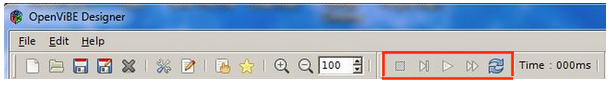
\includegraphics[height=2cm]{images/interface_simu_ov.png}
	\caption{Interface de contrôle de la simulation sous OpenViBE.}
	\label{fig:interface_simu_ov_1}
\end{figure}

\subsubsection*{Description de l'interface du répertoire des blocs fonctionnels}

La partie située à droite de l'interface graphique du designer permet de rechercher des blocs fonctionnels afin de construire un scénario. Ceux-ci sont triés en différentes catégories. un simple glisser-déposer permet de placer un bloc dans l'espace de travail (Figure : \ref{fig:interface_bloc_ov_1}).

\begin{figure}[h]
	\centering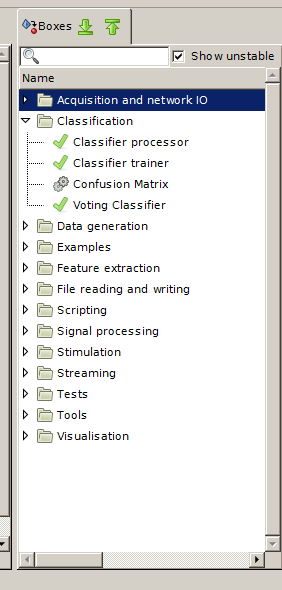
\includegraphics[height=7cm]{images/interface_bloc_ov.png}
	\caption{Interface du répertoire des blocs OpenViBE.}
	\label{fig:interface_bloc_ov_1}
\end{figure}

\subsubsection*{Description de l'espace de travail}

La partie centrale de l'interface graphique correspond à l'espace de travail d'OpenViBE. C'est ici où l'on construit les différents scénarios de l'interface cerveau-ordinateur, via des blocs fonctionnels. Chaque bloc peut être relié à un autre. On peut seulement connecter une entrée à une sortie du même type (e.g. une entrée de type "signal" vers une sortie de type "signal") (Figure : \ref{fig:interface_travail_ov_1}).

\begin{figure}[h]
	\centering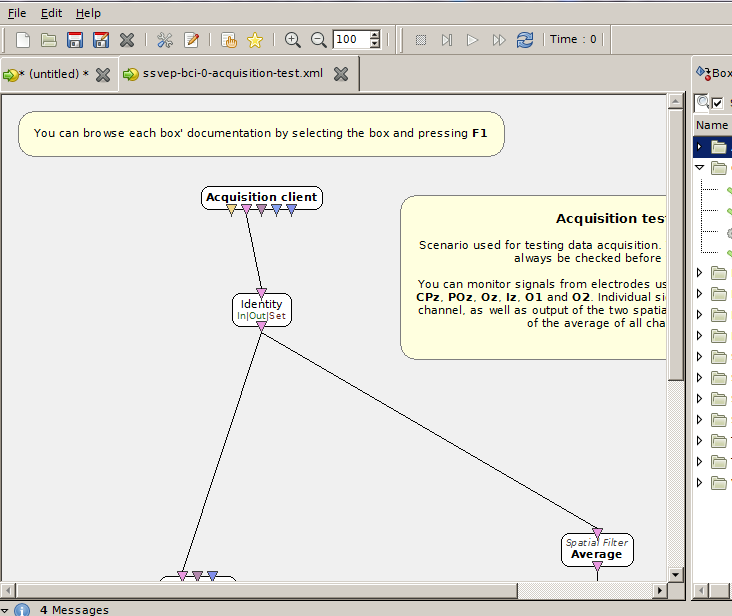
\includegraphics[height=8cm]{images/interface_travail_ov.png}
	\caption{Espace de travail d'OpenViBE.}
	\label{fig:interface_travail_ov_1}
\end{figure}


\newpage
\section*{Manipulation}

\begin{enumerate}
	\smallbreak
	\item Commencez par télécharger et installer OpenViBE.
	\smallbreak
	\item Une fois OpenViBE installé, ouvrez le fichier "online-neuroscience.xml". Il s'agit du scénario comprenant la chaîne de traitement des signaux EEG. 
	\smallbreak
	\item Double-cliquez sur le bloc "Generic Stream Reader" et indiquez le chemin vers le fichier "motor-imagery-csp.ov" qui vous a été fourni. 
	\smallbreak
	\item Double-cliquez sur le bloc "csp-spatial-filter.cfg" et indiquez le chemin vers le fichier csp-spatial-filter.cfg" qui vous a été fourni. 
	\smallbreak
	\item Double-cliquez sur le bloc "Classifier Processor" et indiquez le chemin vers le fichier "classifier.cfg" qui vous a été fourni.
	\smallbreak
	\item Double-cliquez sur le bloc "Graz motor imagery bci simulator" et indiquez le chemin vers le fichier "motor-imagery-bci-graz-stimulator.lua" qui vous a été fourni.
	\smallbreak
	\item Démarrez l'interface cerveau-ordinateur en cliquant sur le bouton "lecture".
\end{enumerate}

\section*{Questions}

\begin{enumerate}
	\smallbreak
	\item Une fois le scénario lancé, aucune activité cérébrale n'apparait dans la fenêtre de visualisation. Le filtre temporel passe-bande a été configuré pour ne laisser passer aucun signal (fréquences de coupures 0Hz, 0Hz). Sachant que l'on souhaite dans le cadre de notre application extraire uniquement certains rythmes du cerveau, comment devez-vous configurer le filtre temporel ? Modifiez la configuration du filtre en double-cliquant dessus. 
	\smallbreak
	\item Quel est le nom des rythmes que l'on souhaite conserver ? 
	\smallbreak
	\item Observez les différentes étapes de traitement des signaux EEG. 
	\smallbreak
	\item L'analyse spectrale des signaux est effectuée avec une FFT. Est-ce la solution la plus optimale ? Pourquoi ? 
	\smallbreak
	\item Proposez une autre solution d'analyse spectrale. 
\end{enumerate}

\newpage
\thispagestyle{fancy}

\begin{center}
	\huge\textbf{GEI 752 : Travail pratique}
	\bigbreak
	\LARGE\textbf{Traitement de signaux EEG et applications dans une interface cerveau-ordinateur}
	\bigbreak
\end{center}

\normalsize

On vous propose à travers ce travail pratique de vous familiariser avec les aspects théoriques et techniques d'une interface cerveau-ordinateur et d'utiliser vos connaissances en traitement du signal afin de participer à la conception de la chaine de traitement des données électroencéphalographiques (EEG).

\newpage
\section*{Interface cerveau-ordinateur}

Une interface Cerveau-Ordinateur ou BCI (Brain Computer Interface) est une interface permettant de réaliser une communication allant du cerveau vers un système numérique (ordinateur par exemple). Pour cela, on s'appuie sur une étude de l'activité neuronale du cerveau grâce à un système électroencéphalographique (EEG) utilisant des électrodes. Celles-ci sont placées à la surface du crâne afin de capter son activité électrique. Un traitement et une analyse des signaux électriques saisis sont réalisés afin de les traduire en informations exploitables par les systèmes numériques. L'expérience que l'on vous propose d'étudier ici s'appuie sur la méthode d'imagerie motrice, qui consiste à imaginer le mouvement de différentes parties du corps. Cela résulte en l'activation du cortex sensorimoteur qui module certains rythmes du cerveau. Ces variations peuvent être détectées par des électrodes EEG. L'interface cerveau-ordinateur en déduit les intentions de l'utilisateur à partir de ces signaux. Dans notre cas, celle-ci doit être capable de déterminer si l'utilisateur pense à un mouvement de sa main droite ou de sa main gauche.

La chaîne de traitement des signaux EEG de l'interface cerveau-ordinateur se compose de 5 étapes (Figure	\ref{fig:interface_travail_ov_5}) : 

\begin{enumerate}
	\item \textbf{L'acquisition des données.} En temps normal, on récupère les données directement issues d'un casque EEG (par exemple le casque EPOC de la société Emotiv). Comme vous ne possédez pas ce genre de casque, on vous fournit un fichier .csv contenant des signaux EEG pré-enregistrés d'une personne pensant aléatoirement à sa main gauche ou droite.
	\smallbreak
	\item \textbf{Filtrage temporel.} Ce filtrage permet d'extraire les rythmes du cerveau qui nous intéressent.
	\smallbreak
	\item \textbf{Filtrage spatial.} On souhait utiliser un filtrage spatial afin d'optimiser nos données. Il vous sera demandé ultérieurement d'implémenter ce filtre sous Matlab. 
	\item \textbf{Filtrage spatial CSP.} Permet de réduire la quantité d'informations à traiter en réalisant une décorrélation et en pondérant certaines des sorties du casque. 
	\smallbreak
	\item \textbf{Analyse spectrale.} Réalise une analyse spectrale via une transformée de Fourier.
	\smallbreak
	\item \textbf{Classification.} Effectue une classification des caractéristiques présentes à son entrée afin de déterminer à quelle main pensait l'utilisateur à un instant donné. 
\end{enumerate}

Le classificateur nécessite d'être préalablement entrainé grâce à d'autres scénarios, qui génèrent alors son fichier de configuration. On vous fournit directement le fichier de configuration ("classifier.cfg"). Veuillez également noter que vous ne possédez pas le scénario d'acquisition permettant de récupérer les données EEG. On vous fournit donc également les données filtrées temporellement dans le fichier ("données\_entrée.csv").

\begin{figure}[h]
	\centering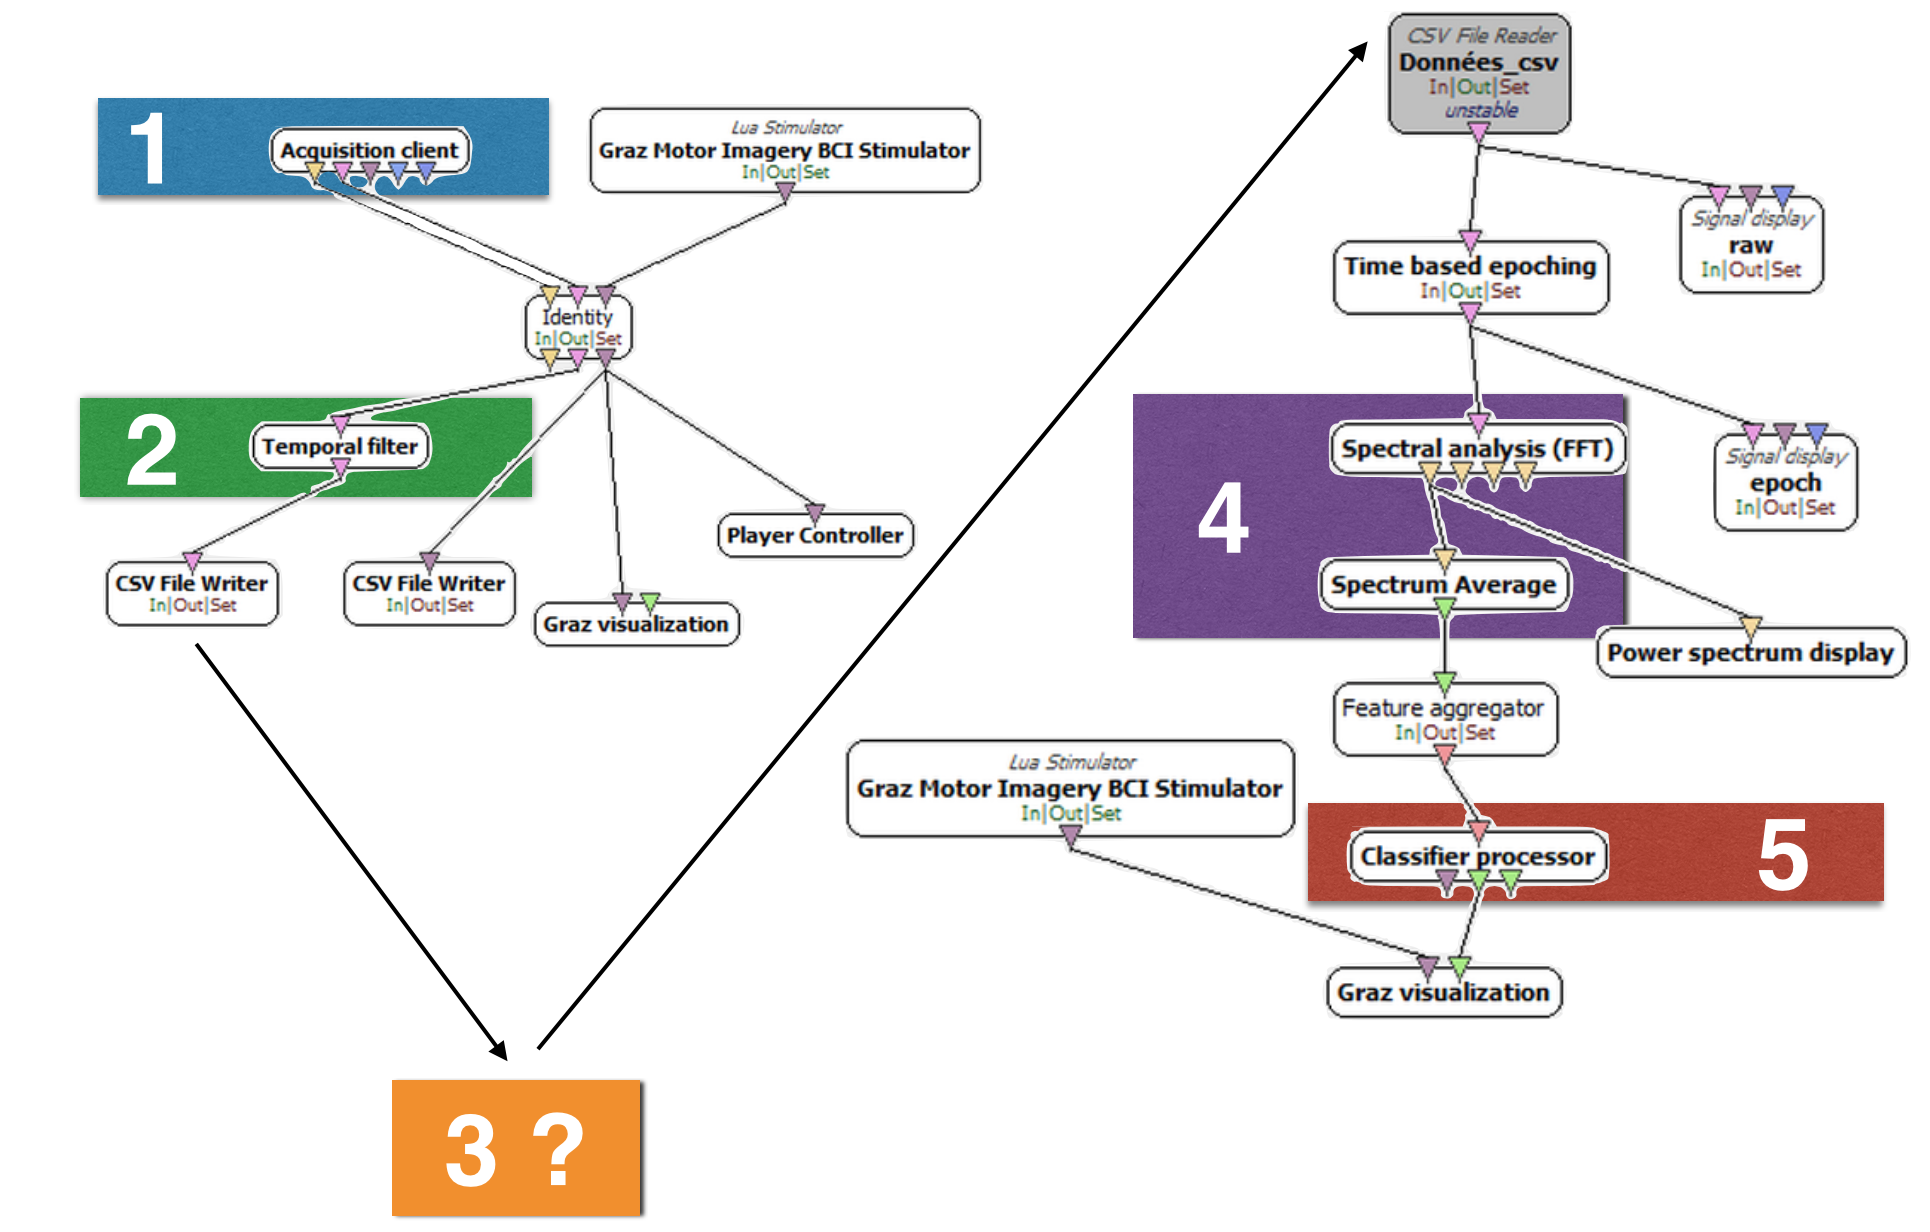
\includegraphics[height=10cm]{images/sujet_signal_color.png}
	\caption{Traitement des signaux EEG sous OpenViBE.}
	\label{fig:interface_travail_ov_5}
\end{figure}

\newpage
\section*{OpenViBE}

\subsection*{Présentation du logiciel}

OpenViBE est une plateforme logicielle dédiée à la conception et à l'utilisation d'interfaces cerveau-ordinateur en temps réel. Celle-ci est éditée par l'Institut National de Recherche en Informatique et en Automatique (INRIA) de Rennes (France). Le logiciel gère à la fois l'acquisition, le traitement et l'analyse des signaux.

Le logiciel fonctionne sous la forme de scénarios, correspondant à un ensemble de blocs fonctionnels. La suite OpenViBE est composée de deux logiciels : 
\begin{itemize}
	\item \textbf{OpenViBE designer}. Il s'agit d'un éditeur de scénario permettant de  créer et modifier les schémas blocs grâce à une interface graphique. Il suffit alors de placer les différents blocs, de les configurer (en cliquant dessus), et de les relier pour former une chaine de traitement.
	\smallbreak
	\item \textbf{OpenViBE acquisition server.} Permet d'acquérir des données EEG brutes à partir de dispositifs EEG. Il est par exemple possible de connecter différents types de casques, dont le casque EPOC.
	\smallbreak
\end{itemize}

\subsection*{Téléchargement et installation d'OpenViBE}

Le logiciel fonctionne sous les systèmes d'exploitations Windows (Windows XP ou ultérieur, la stabilité du logiciel sous Windows 8 n'ayant pas été vérifiée par l'éditeur) et Linux (Ubuntu, Fedora). La liste détaillée des architectures compatibles avec OpenViBE est disponible à l'adresse suivante : http://openvibe.inria.fr/supported-architectures/.
Il est possible de télécharger l'installeur OpenViBE à l'adresse suivante : http://openvibe.inria.fr/downloads/. Une fois celui-ci téléchargé, il suffit de l'ouvrir et de suivre les indications affichées à l'écran.

\subsection*{Présentation de l'interface utilisateur d'OpenViBE Designer}

\subsubsection*{Description de l'interface de contrôle de la simulation}

La partie supérieure de l'interface graphique permet de contrôler la simulation, i.e. le déroulement du scénario. Ainsi, il est possible de lancer un scénario en appuyant sur le bouton "lecture", de le stopper en appuyant sur le bouton "stop" et d'en accélérer le déroulement en appuyant sur le bouton "avance rapide". Il est également possible de lancer plusieurs scénarios en même temps (Figure : \ref{fig:interface_simu_ov_2}). 

\begin{figure}[h]
	\centering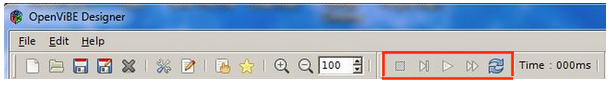
\includegraphics[height=2cm]{images/interface_simu_ov.png}
	\caption{Interface de contrôle de la simulation sous OpenViBE.}
	\label{fig:interface_simu_ov_2}
\end{figure}

\subsubsection*{Description de l'interface du répertoire des blocs fonctionnels}

La partie située à droite de l'interface graphique du designer permet de rechercher les blocs afin de construire un scénario. Ceux-ci sont triés en différentes catégories. un simple glisser-déposer permet de placer un bloc dans l'espace de travail (Figure : \ref{fig:interface_bloc_ov_2}).

\begin{figure}[h]
	\centering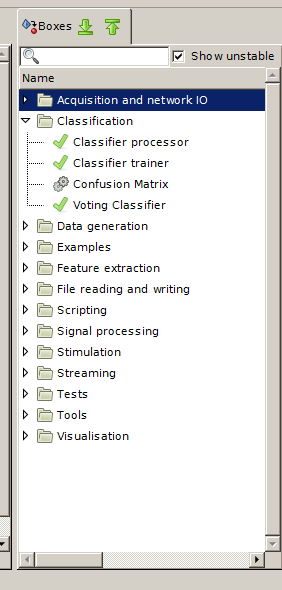
\includegraphics[height=7cm]{images/interface_bloc_ov.png}
	\caption{Interface du répertoire des blocs OpenViBE.}
	\label{fig:interface_bloc_ov_2}
\end{figure}

\subsubsection*{Description de l'espace de travail}

La partie centrale de l'interface graphique correspond à l'espace de travail d'OpenViBE. C'est ici que l'on construit les différents scénarios de l'interface cerveau-ordinateur, via des blocs fonctionnels. Chaque bloc peut être relié à un autre. On peut seulement connecter une entrée à une sortie du même type (e.g. une entrée de type "signal" vers une sortie de type "signal") (Figure : \ref{fig:interface_travail_ov_4}).

\begin{figure}[h]
	\centering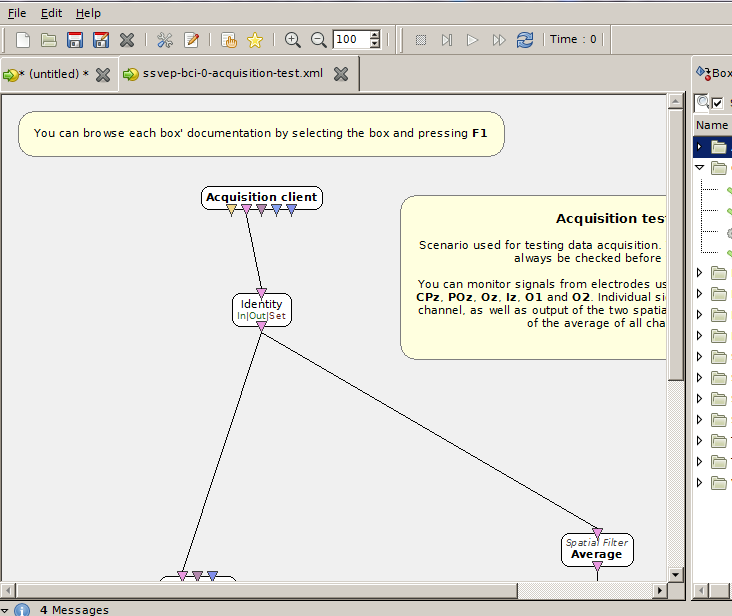
\includegraphics[height=8cm]{images/interface_travail_ov.png}
	\caption{Espace de travail d'OpenViBE.}
	\label{fig:interface_travail_ov_4}
\end{figure}


\newpage

\section*{Manipulation}

\begin{enumerate}
	\smallbreak
	\item Commencez dans un premier temps par télécharger et installer OpenViBE. Celui-ci vous servira dans la question 3. 
	\smallbreak
	\item On vous demande de coder un filtre spatial PCA sous Matlab et de traiter les données EEG contenues dans le fichier "données\_entrée.csv". Le code Matlab n'étant pas directement exécutable dans OpenViBE, vous devez utiliser la fonction Matlab "lecture\_csv.m" afin d'extraire les données EEG du fichier "données\_entrée.csv", ainsi que la fonction "ecriture\_csv.m" afin d'écrire les données après filtrage spatial vers le fichier CSV "données\_EEG\_sortie.csv".
	\smallbreak
	\item Une fois le code implémenté et vos données filtrées, on exporte les signaux vers OpenViBE. Pour cela, démarrez OpenViBE. Ouvrez ensuite le fichier "online.xml".
	\smallbreak
	\item Double-cliquez sur le bloc "CSV File Reader" et indiquez le chemin vers le fichier que vous avez généré à partir de votre code Maltab. Par défaut, ce fichier s'appelle "données\_EEG\_sortie.csv". 
	\smallbreak
	\item Double-cliquez sur le bloc "Classifier Processor" et indiquez le chemin vers le fichier "classifier.cfg" qui vous a été fourni.
	\smallbreak
	\item Double-cliquez sur le bloc "Graz motor imagery bci simulator" et indiquez le chemin vers le fichier "motor-imagery-bci-graz-stimulator.lua" qui vous a été fourni.
	\smallbreak
	\item Démarrez l'interface cerveau-ordinateur en cliquant sur le bouton "lecture". Qu'observez vous dans la fenêtre de visualisation ? 
	\smallbreak 
	\item De la même manière que dans la question 2, on vous demande à présent d'implémenter un filtre spatial ICA sous Matlab. Exportez de nouveau vos données vers OpenViBE. Qu'observez vous ? 
\end{enumerate}



\newpage



%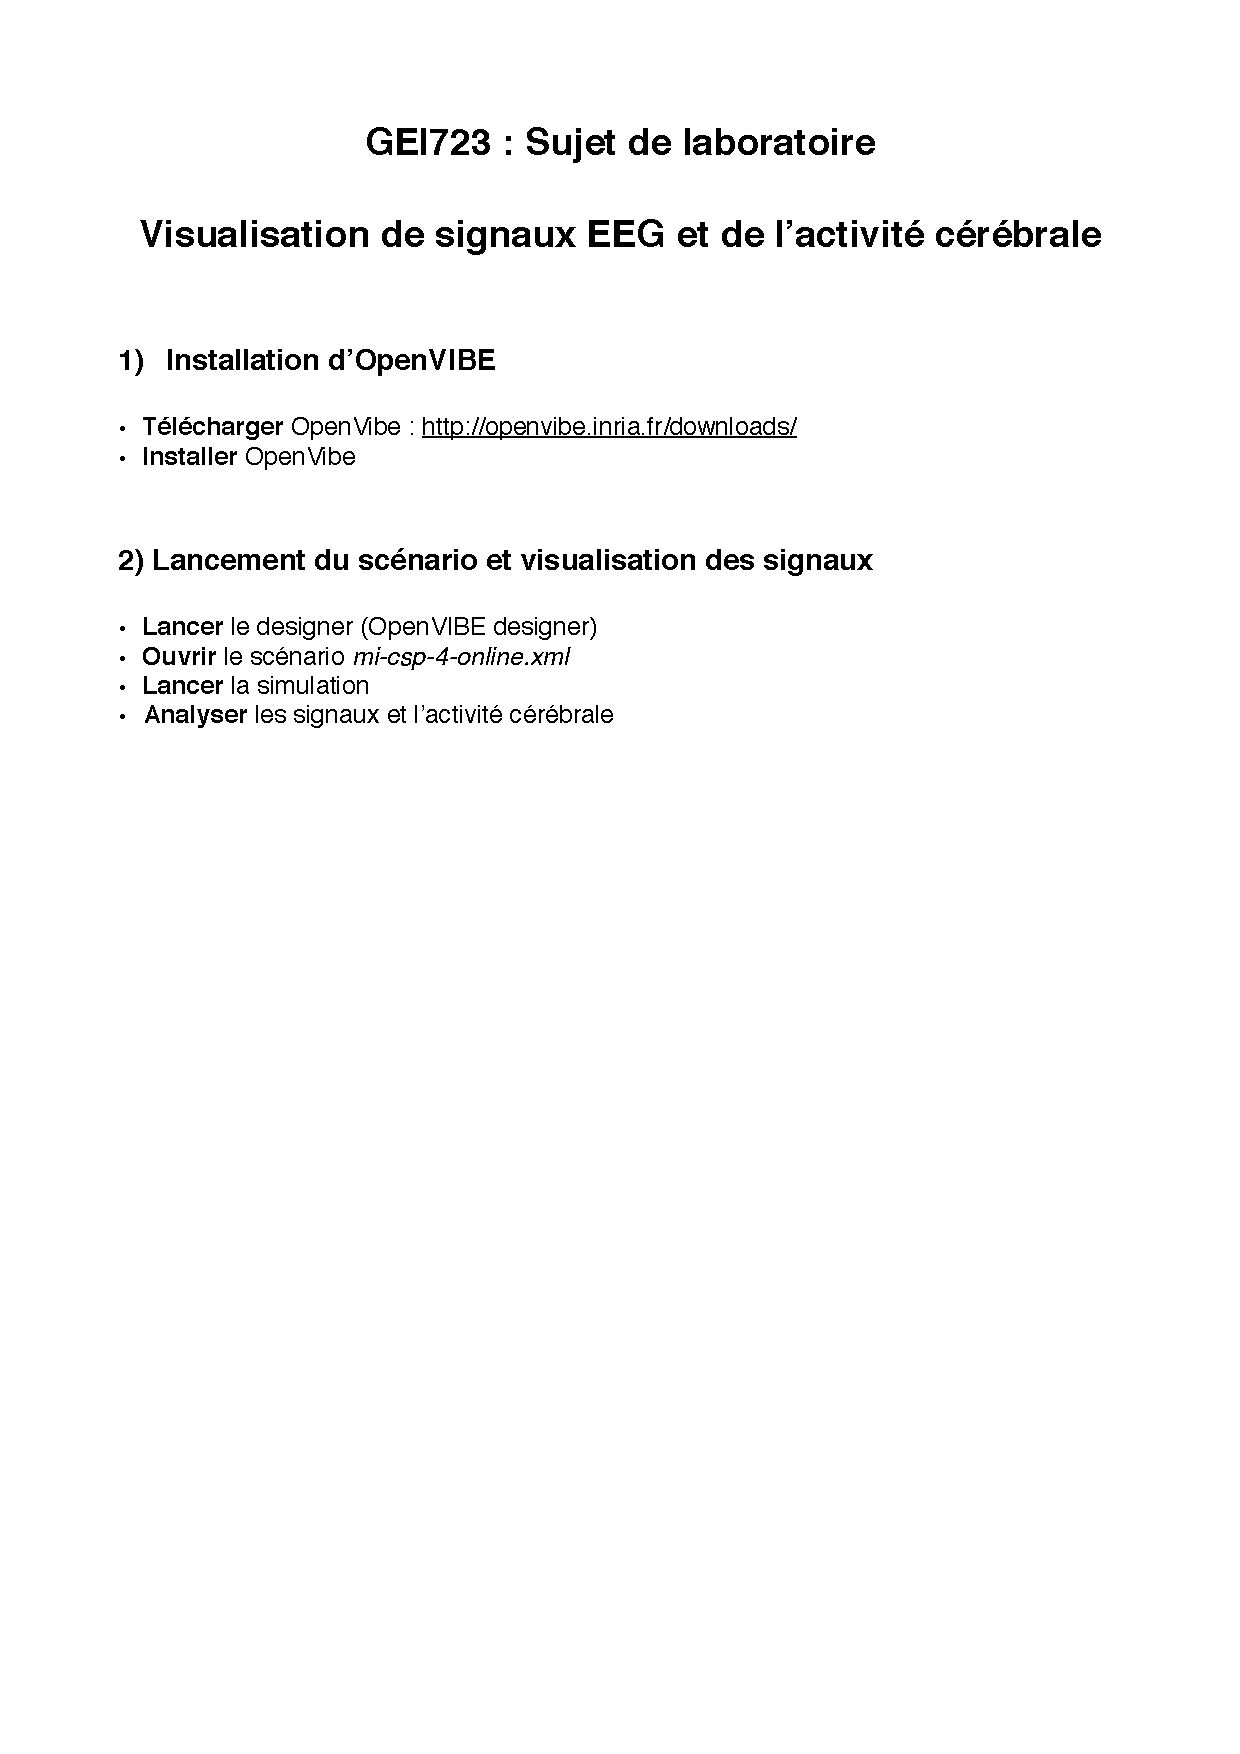
\includepdf[pages=1]{pdf/Sujet_GEI723.pdf}